\section{System Model}
%----------------------------------------------------------------------------------------%
\subsection{Network Model}
We consider an edge computing system with $K$ Access Points (APs) and $M$ edge servers, which are connected in a network as illustrated in Fig.\ref{fig:system}.
The sets of APs and edge servers are denoted as $\apSet \define \set{1,\dots,K}$ and $\esSet \define \set{1,\dots,M}$, respectively.
\accept{
    Without loss of generality, it is assumed that there are $J$ types of computation jobs supported in this system, which are denoted via the $\mathcal{J} \define \set{1,\dots,J}$.
}
Each AP collects the computation jobs from the mobile users within its coverage, and makes decision on the processing edge servers for each job type from the set $\esSet$.
It is assumed that the $k$-th AP only dispatches the computation jobs to the edge servers \fixit{within a certain number of hops.}
Let $\esSet_{k} \subseteq \esSet$ be the set of edge servers, which can compute the jobs from the $k$-th AP;
and $\ccSet_{k}$ be the set of APs, which may upload jobs to the $m$-th edge server.
We refer to $\esSet_{k}$ as the \emph{cadidate server set} of the $k$-th AP, and $\apSet_{m}$ as the \emph{candidate AP set} of the $m$-th edge server.
As illustrated in Fig.\ref{fig:conflict}, different APs may have different candidate server ser according to their locations in the network.
For example, it is possible that $\esSet_{k} \neq \esSet_{k'}$ and $\esSet_{k} \cap \esSet_{k'} \neq \emptyset$ when $k \neq k' \in \apSet$.
In this edge computing network, we shall focus on the decentralized dispatcher design at each AP.
Specifically, each AP and edge server periodically broadcast their state information (e.g. edge server dispatching choice for each job type, list of jobs being uploaded from APs to edge servers, computing queue length and etc.), and one AP updates its strategy on job dispatching when receiving the broadcast state information.
\comment{
    In this paper, we shall optimize the job dispatching strategy at APs with part of the broadcast information and random broadcast latency.
}

\begin{figure}[ht]
    \centering
    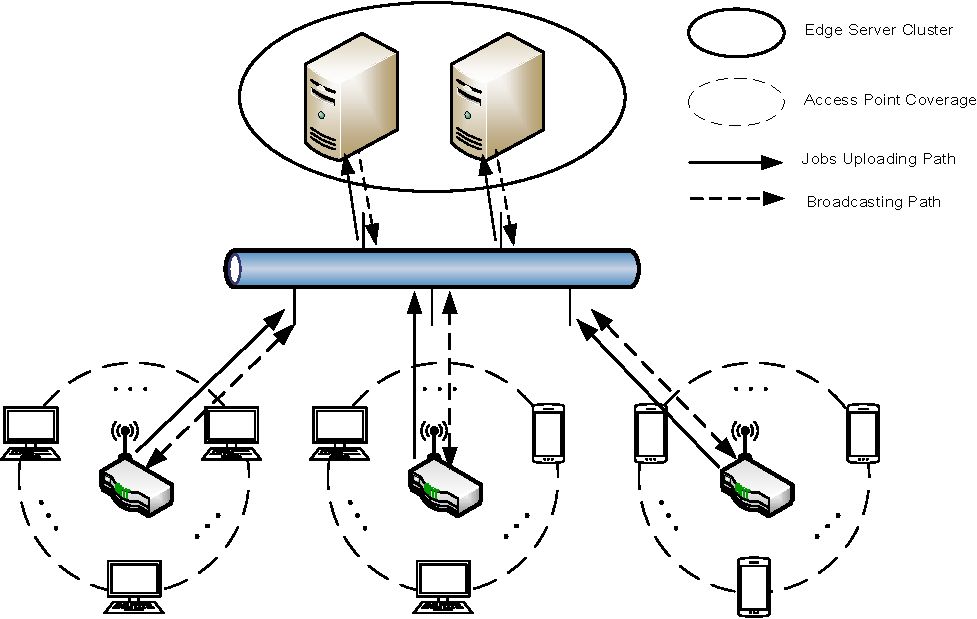
\includegraphics[width=0.80\textwidth]{system-model.pdf}
    \caption{The Illustration of MEC System Model}
    \label{fig:system}
\end{figure}

%NOTE: [job space support and arrival process]
The time axis is organized by time slots.
The job arrivals in each time slot at each AP are modelled via independent Bernoulli distributions.
Specifically, the arrivals of the $j$-th job type at the $k$-th AP in different time slots are independent and identically distributed (i.i.d) Bernoulli random variables, and the arrival probability is denoted as $\lambda_{k,j}$ ($\forall k\in\apSet, j\in\jSpace$).
Let $A_{k,j}(t) \in \set{0,1}$ represents the event of job arrival, where $A_{k,j}(t)=1$ means one job of the $j$-th job type arrives on the $k$-th at the $t$-th time slot, and $A_{k,j}(t)=0$ means other wise.
Hence,
\begin{align}
    \Pr\{ A_{k,j}(t) = 1 \} = \lambda_{k,j}, \forall k,j,t
\end{align}

%NOTE: [uploading process]
Each AP then immediately dispatches each type of received jobs to one edge server.
Let $\omega_{k,j} \in \esSet_{k}$ denotes the index of edge server for processing of the $j$-th job type dispatched from the $k$-th AP ($\forall k\in\apSet, j\in\jSpace$).
Different types of jobs may have different distributions on the input data size.
Moreover, due to the random traffic in the network, the job uploading from one AP to one edge server consumes a random number of time slots.
It's assumed that the distributions of uploading time are independent between any two uploading jobs.
Hence, we denote $\mathcal{U}_{k,m,j}$ as the uploading time for the $j$-th job type uploading from the $k$-th AP to the $m$-th edge server following some distribution with support $\set{1, \dots, \Xi}$, where $\Xi$ denotes the maximum uploading time ($\forall k\in\apSet, m\in\esSet, j\in\jSpace$).
In practice, the distribution of uploading latency may not be known to the APs or edge servers in advance.

%NOTE: [processing process]
There are $J$ virtual machines (VMs) on each edge server for the computation of $J$ job types, respectively.
For each type, the uploaded jobs are computed in a First-Come-First-Serve (FCFS) manner.
Hence, a processing queue with maximum $L_{max}$ jobs is established for each VM.
The arrival jobs will be discarded when the processing queue is full.
Furthermore, we adopt the \emph{unrelated machines} assumption in \cite{tan-online} for job processing on edge servers.
Specifically, it is assumed that the computation time of different job types on different edge servers follows the memory-less Geometric distribution with different expectations.
\fixit{
    Let $C_{m,j} \sim \mathbb{G}(1/c_{m,j})$ be the computation time distribution (with the unit of time slot) of the $j$-th job type on the $m$-th edge server, where $c_{m,j}$ is the expectation.
}
Hence, the probability mass function (PMF) of $C_{m,j}$ is given by:
\begin{align}
    f_{m,j}(k) \define (1-\frac{1}{c_{m,j}})^{k-1} \frac{1}{c_{m,j}}.
\end{align}
%----------------------------------------------------------------------------------------%

\subsection{Periodic Broadcast of State Information}
%NOTE: Periodic Broadcast is Indispensable
In order to facilitate cooperatice dispatching for the APs, it is assumed that all the APs and edge servers will broadcast their local state information (LSI) every $t_B$ time slots as depicted in Fig.\ref{fig:brd-timeline}.
We shall refer to every $t_B$ time slots as a broadcast interval.
At the beginning of each broadcast interval (say the $t$-th broadcast interval), the LSI of each AP and edge server is defined below.

\begin{figure}[ht]
    \centering
    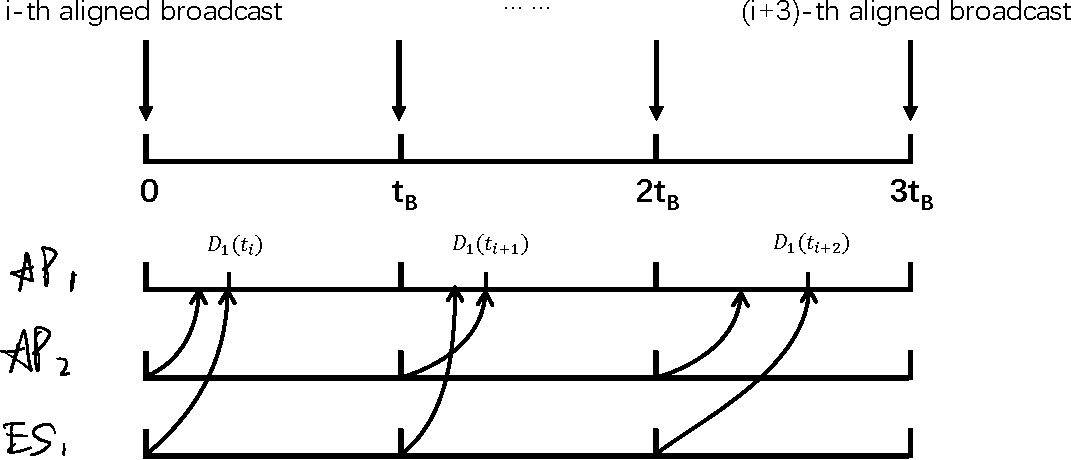
\includegraphics[width=0.80\textwidth]{brd-timeline.pdf}
    \caption{The Timeline Illustration of State Information Broadcast and Receiving}
    \label{fig:brd-timeline}
\end{figure}

%NOTE: State and Broadcast Information for AP
One AP shall maintain information about the number of jobs still in uploading. 
And due to the uploading time of one job is unknown until it's been uploaded, it further has counters to record the elapsed time slots for each job.
More specifically, at the $n$ time slot in the $t$-th interval, the number of the $j$-th type job been uploaded to the $m$-th edge server $\xi$ time slots ago from $k$-th AP is denoted as $R^{(k)}_{m,j,\xi}({t,n})$ ($\forall k\in\apSet, m\in\esSet, j\in\jSpace, \xi\in(0,\Xi]$).
The broadcast information of the $k$-th AP at the $t$-th broadcast includes the information about uploading job and the dispatching decision for each type of jobs, which is defined as follows.
\accept{
    \begin{align}
        \mathcal{R}_{k}({t}) \define \set{\vec{R}^{(k)}_{m,j}({t}), \set{\omega_{k,j}(t)|\forall j\in\jSpace} | \forall m\in\esSet, j\in\jSpace},
    \end{align}
}
where $\vec{R}^{(k)}_{m,j} \define ( R^{(k)}_{m,j,0},\dots,R^{(k)}_{m,j,\Xi} )$ denotes the vector of random variables for convenience.

%NOTE: State and Broadcast Information for ES
One edge server shall maintain information about the computing queue status for each VM.
\accept{
    More specifically, at the $n$ time slot in the $t$-th interval, the $m$-th edge server have $Q_{m,j}({t,n})$ denote the pending number of the $j$-th type job ($\forall m\in\esSet, j\in\jSpace$).
    The broadcast information of the $m$-th edge server at the $t$-th ($t\in\domZ$) broadcast is defined as follows.
    \begin{align}
        \mathcal{Q}_{m}({t}) \define \set{Q_{m,j}({t}) | \forall j\in\jSpace}.
    \end{align}
    And the whole broadcast information from all APs and edge servers at the $i$-th broadcast ($i\in\domZ$) is denoted as:
    \begin{align}
        \Obsv^{\dagger}(t) \define
            \Brace{
                \mathcal{R}_{k}({t}), \mathcal{Q}_{m}({t}) | \forall k\in\apSet, m\in\esSet
            },
    \end{align}
}

%NOTE: Conflict of AP set and partial information definition
\begin{figure}[ht]
    \centering
    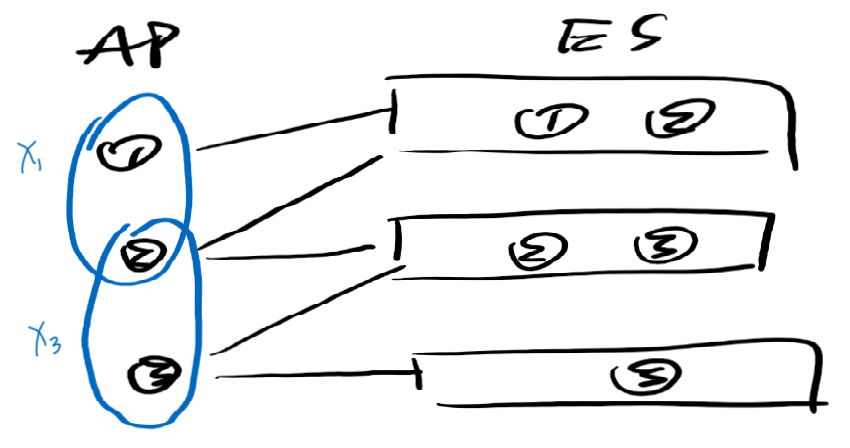
\includegraphics[width=0.80\textwidth]{images/draft-conflict.png}
    \caption{The Example Illustraction of Conflict Set and Partial Broadcast Information}
    \label{fig:conflict}
\end{figure}

In a \fixit{large-scale edge computing network}, it may not be feasible for each AP to collect the LSI from all other APs and edge servers.
Hence, we first define the \emph{conflict AP set} as follows.
\begin{align}
    \ccSet_{k} \define \bigcup_{m\in\esSet_{k}} \apSet_{m}
    % \ccSet_{k} \define \set{\forall k' \neq k\in\apSet|\esSet_{k'} \cap \esSet_{k} \neq \emptyset}
\end{align}
\fixit{The \emph{conflict set} indicates the subset of APs whose status information could affect the decision making for the $k$-th AP.}
It is assumed that each AP can only collect the LSI from the APs in its \emph{conflict AP set} and edge servers from its \emph{candidate server set}.
Hence, we can define the observed state information (OSI) of the $k$-th AP as follows.
\begin{align}
    \Obsv_{k} &= \set{\mathcal{R}_{k'} | \forall k'\in\ccSet_{k}}
                    \cup \set{\mathcal{Q}_{m} | \forall m\in\esSet_{k}},
\end{align}

Moreover, the transimission latency of LSI in a \fixit{large-scale edge computing network} is not negligible.
It is assumed that the $k$-th AP is able to collect the OSI $D_{k}(t)$ time slots after the broadcast of the $t$-th interval.
$D_{k}(t)$ is a random variable follows some distribution with support $\set{1,\dots,t_B}$, i.e. the broadcast interval $t_B$ is set that the $k$-th AP \fixit{could receive one broadcast information before the next interval}.

One AP will update its dispatching decision after the reception of its OSI.
Specifically, let $\omega_{k,j}(t)$ be the new computing edge server for the $t$-the broadcast interval, the $k$-th AP should determine th new policy in the $D_{k}(t)$ time slot of the $t$-th broadcast interval.

\fixit{
    According to Fig.\ref{fig:brd-timeline}, different APs would receive different parts of broadcast information at different time slots.
    Specifically, each AP would require only partial broadcast information to help it make dispatching decision.

    For the $t$-th broadcast, the $k$-th AP would receive the partial broadcast information $\Obsv_{k}(t)$ after some latency which is denoted as \brdelay~$D_{k}(t)$.
    Due to the randomness of the network traffic, the \brdelay~shall be random based on the uncertainty of the arrival latency of each part of information from \emph{candidate set} of edge servers and \emph{conflict set} of APs.
    Thus the probability distributions of \brdelay~ are i.i.d random variables following some distributions.

    As a high frequency broadcast design could result into \emph{broadcast storm} and block the normal network traffic, we introduce a slow enough broadcast interval selection in the system.
    The broadcast interval is always larger than the maximum \brdelay, i.e. $t_B > \hat{D}_k$ ($\forall k\in\apSet$), where $\hat{D}_k$ is the upper bound for $D_{k}({t})$ ($t\in\domP$).
    The broadcast interval selected implies that any AP would always receive the whole broadcast information once before the next broadcast, and the \brdelay~is comparable to the broadcast interval thus not negligible.

    Each AP tries to update its dispatching decisions once it receives partial broadcast information.
    Denote the individual dispatching policy of the $k$-th AP ($\forall k\in\apSet$) based on the broadcast information $\Obsv_{k}({t})$ ($t \in\domP$) as follows.
    \begin{align}
        &\Omega_{k}(\Obsv_{k}(t)) \define \set{\omega_{k,j}|\forall m\in\esSet, j\in\jSpace}.
        \label{def_action}
    \end{align}
    And we note that the $k$-th AP would always adopt two phases polices in the $t$-th interval, i.e. $\Omega_{k}(\Obsv_{k}({t-1}))$ before receiving $\Obsv_{k}(t)$ and $\Omega_{k}(\Obsv_{k}(t))$ afterwards.
    % The two phases policy of APs in one together determine the transition of $\Obsv({t+1})$ in the next interval.
}

However, the randomness of \brdelay~implies that one AP could not know other APs' \brdelay~in the same interval.
Thus, APs are unable to evaluate the impact introduced by others' policy on the next broadcast information and fail to establish exact cooperation.
An naive way to solve this problem is to force all APs update their policy only at the end of the interval, which introduces a inevitable lagging for a whole broadcast interval.
\delete{v4}{A toy example is given as follow.}

In the following problem formulation section, we will show that we could come up with better dispatching decision update solution which is aware of the \brdelay, and improve APs' dispatching decisions in an iterative way.
\accept{
    Furthermore, with the help of algorithm design we could prove that our improved policy is with analytical performance bound under MDP framework.
}

\delete{v6.1}{
    One simple example is given as follows.
    \begin{example}
        As depicted in \ref{fig:conflict}, there are 3 APs and 3 edge servers in the system.
        The \emph{candidate set} for each AP is denoted as: $\esSet_{1}=\set{1}, \esSet_{2}=\set{1,2}, \esSet_{3}=\set{2,3}$, respectively.
        The \emph{conflict set} for each AP is denoted as: $\ccSet_{1}=\set{1,2}, \ccSet_{2}=\set{1,2,3}, \ccSet_{3}=\set{2,3}$.
        And the partial information required for each AP is denoted as follows.
        \begin{align*}
            \Obsv_{1} &= \set{ \mathcal{R}_{2} } \cup \set{ \mathcal{Q}_{1} }
            \\
            \Obsv_{3} &= \set{ \mathcal{R}_{2} } \cup \set{ \mathcal{Q}_{2}, \mathcal{Q}_{3} }
        \end{align*}
        % And we note that
    \end{example}
}
%----------------------------------------------------------------------------------------%